\subsection{Determining upper and lower bound support}

Because the total number of possible rules extracted
from a data set grows exponentially it is necessary to find a minimum support count so we don't have to waste computational power in finding uninteresting and obvious rules.
We want to find rules with relatively low support and high confidence.
We run the apriori algorithm and let weka generate output itemsets for us.  We copy the one itemset frequency list into excel and generate the following table.


\begin{figure}[H]
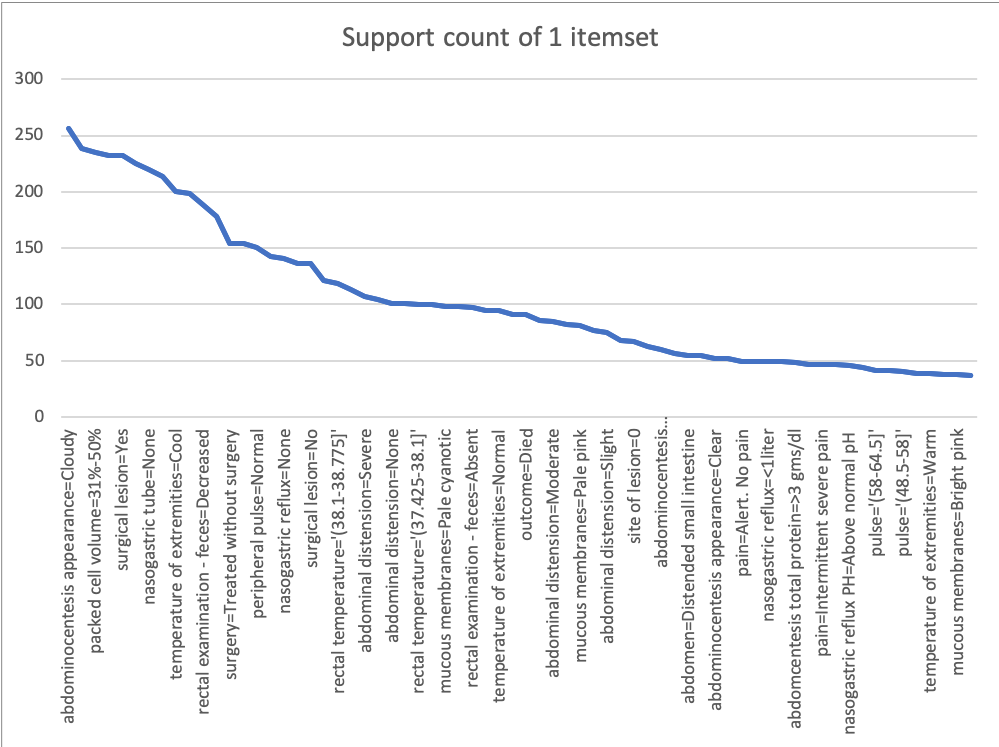
\includegraphics[scale=0.7]{SupportCountTable.png}

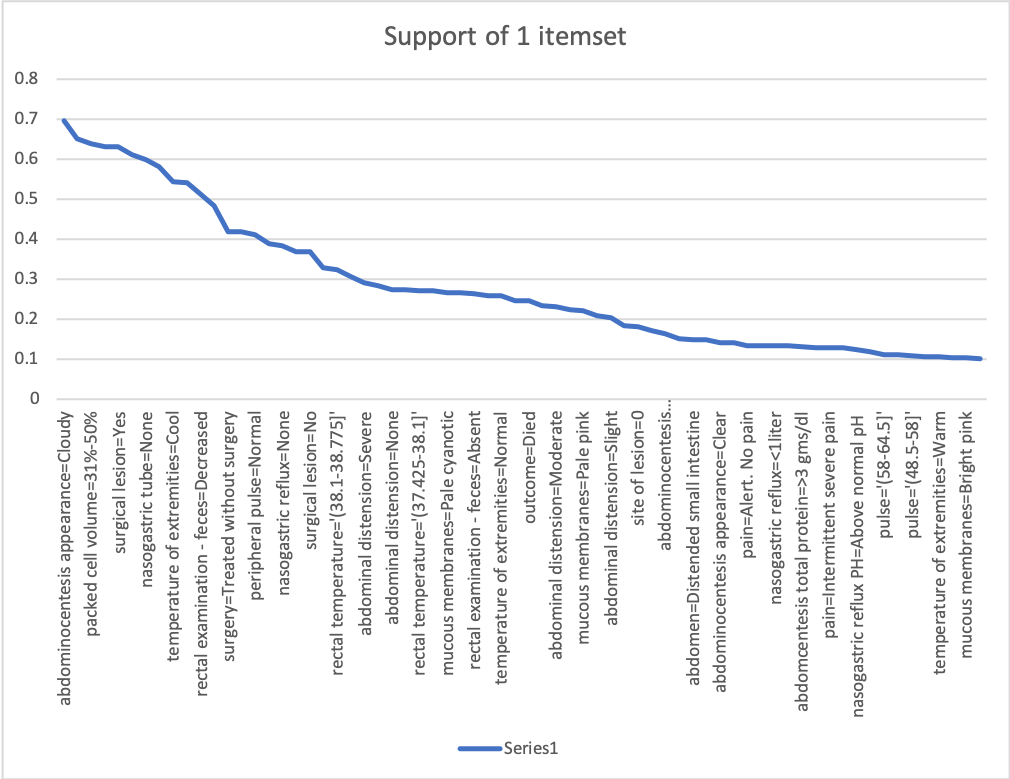
\includegraphics[scale=0.7]{SupportTable.png}
\end{figure}

We deduct from the table that the most interesting rules will have support level of less than 0.42 since any rule with more support than that will probably be rather obvious. So we set the upperBoundMinSupport to 0.42 in the Associate settings.\\
Since there are no itemset with support lower than 0.1 we can set the lowerBoundMinSupport to 0.1.